\chapter{Inner Product Geometry}
\label{ch:inner-product-geometry}

\section{Why Geometry Has To Be Added}

A vector space remembers addition and scalar multiplication. That is enough to
talk about span, bases, coordinates, kernels, and images. It is not enough to
talk about length, angle, similarity, or error.

Those words require extra structure. In data problems this extra structure is
not cosmetic. If two documents are represented by vectors, their ``similarity''
usually means an angle or a normalized dot product. If a model makes prediction
errors, the size of the error usually means a norm. If an equation has no exact
solution, the phrase ``best approximate solution'' only makes sense after we
choose a way to measure distance.

\begin{aimlbox}
This chapter is not about a particular machine-learning algorithm. It builds
the geometry that later lets us say precise things about regression, PCA,
orthogonal features, residuals, and numerical error. The point is to make
linear algebra ready for data, not to turn every theorem into an application.
\end{aimlbox}

\section{Inner Products}

\begin{definition}[Inner product]
Let $V$ be a real vector space. An \emph{inner product} on $V$ is a rule
\[
  \inner{\cdot}{\cdot}: V \times V \to \R
\]
satisfying, for all $u,v,w \in V$ and $\lambda \in \R$,
\begin{enumerate}[label=(\alph*)]
  \item \textbf{positivity:} $\inner{v}{v} \geq 0$, and
        $\inner{v}{v}=0$ if and only if $v=0$;
  \item \textbf{linearity in the first slot:}
        $\inner{u+v}{w}=\inner{u}{w}+\inner{v}{w}$ and
        $\inner{\lambda u}{w}=\lambda\inner{u}{w}$;
  \item \textbf{symmetry:} $\inner{u}{v}=\inner{v}{u}$.
\end{enumerate}
An \emph{inner product space} is a vector space equipped with an inner
product.
\end{definition}

In this course the main example is the standard dot product on $\R^n$:
\[
  \inner{x}{y}
  = x^T y
  = x_1y_1 + x_2y_2 + \cdots + x_ny_n.
\]
The axioms are worth naming because the same algebraic rules work in spaces of
polynomials, matrices, functions, and signals, even when the vectors are not
drawn as arrows.

\begin{example}[Weighted dot product]
Let $c_1,\ldots,c_n$ be positive numbers. Then
\[
  \inner{x}{y}_c = c_1x_1y_1+\cdots+c_nx_ny_n
\]
is an inner product on $\R^n$. Coordinates with larger weights count more in
the geometry. This is the linear-algebraic beginning of weighted least squares:
some measurement errors may matter more than others.
\end{example}

\begin{example}[Matrix inner product]
For $m \times n$ real matrices, define
\[
  \inner{A}{B} = \sum_{i=1}^m \sum_{j=1}^n A_{ij}B_{ij}.
\]
This is just the dot product after stacking the entries into one long vector.
It is often called the Frobenius inner product.
\end{example}

\begin{example}[Polynomial inner product]
On polynomials of degree at most $d$, one possible inner product is
\[
  \inner{p}{q} = \int_{-1}^{1} p(t)q(t)\,dt.
\]
Another possible inner product is the coefficient dot product:
if $p(t)=a_0+a_1t+\cdots+a_dt^d$ and
$q(t)=b_0+b_1t+\cdots+b_dt^d$, set
\[
  \inner{p}{q}_{\mathrm{coef}} = a_0b_0+\cdots+a_db_d.
\]
These are different geometries on the same vector space.
\end{example}

\begin{warningbox}
The vector space does not determine the inner product. The same vectors may
have different lengths and angles under different inner products. In
applications, choosing the inner product is part of choosing what counts as
similar, large, small, or costly.
\end{warningbox}

\section{Norms, Distance, and Orthogonality}

\begin{definition}[Norm induced by an inner product]
If $V$ is an inner product space, the induced norm is
\[
  \norm{v} = \sqrt{\inner{v}{v}}.
\]
The distance between $u$ and $v$ is
\[
  \dist(u,v)=\norm{u-v}.
\]
\end{definition}

\begin{proposition}[Basic norm properties]
For all $u,v \in V$ and $\lambda \in \R$,
\[
  \norm{v}\geq 0,\qquad
  \norm{v}=0 \Longleftrightarrow v=0,\qquad
  \norm{\lambda v}=|\lambda|\,\norm{v}.
\]
\end{proposition}

\begin{proof}
The first two statements are exactly positivity of the inner product. For the
scaling rule,
\[
  \norm{\lambda v}^2
  = \inner{\lambda v}{\lambda v}
  = \lambda^2\inner{v}{v}
  = |\lambda|^2\norm{v}^2.
\]
Taking square roots gives the result.
\end{proof}

\begin{definition}[Orthogonality]
Vectors $u$ and $v$ are \emph{orthogonal}, written $u \perp v$, if
\[
  \inner{u}{v}=0.
\]
\end{definition}

Orthogonality is the algebraic version of a right angle. The definition makes
sense whether the vectors are arrows, coefficient lists, images, or error
signals.

\begin{theorem}[Pythagorean theorem]
If $u \perp v$, then
\[
  \norm{u+v}^2=\norm{u}^2+\norm{v}^2.
\]
\end{theorem}

\begin{proof}
\[
\begin{aligned}
  \norm{u+v}^2
  &= \inner{u+v}{u+v} \\
  &= \inner{u}{u}+\inner{u}{v}+\inner{v}{u}+\inner{v}{v} \\
  &= \norm{u}^2 + 0 + 0 + \norm{v}^2.
\end{aligned}
\]
\end{proof}

\section{Projection Onto A Line}

Projection is the basic move behind least squares. Before projecting onto a
large subspace, we should understand projection onto a single line.

\begin{definition}[Projection onto a nonzero vector]
Let $v \neq 0$. The projection of $u$ onto the line spanned by $v$ is
\[
  \Proj_v(u)=\frac{\inner{u}{v}}{\inner{v}{v}}\,v.
\]
The residual is
\[
  r = u-\Proj_v(u).
\]
\end{definition}

\begin{figure}[htbp]
  \centering
  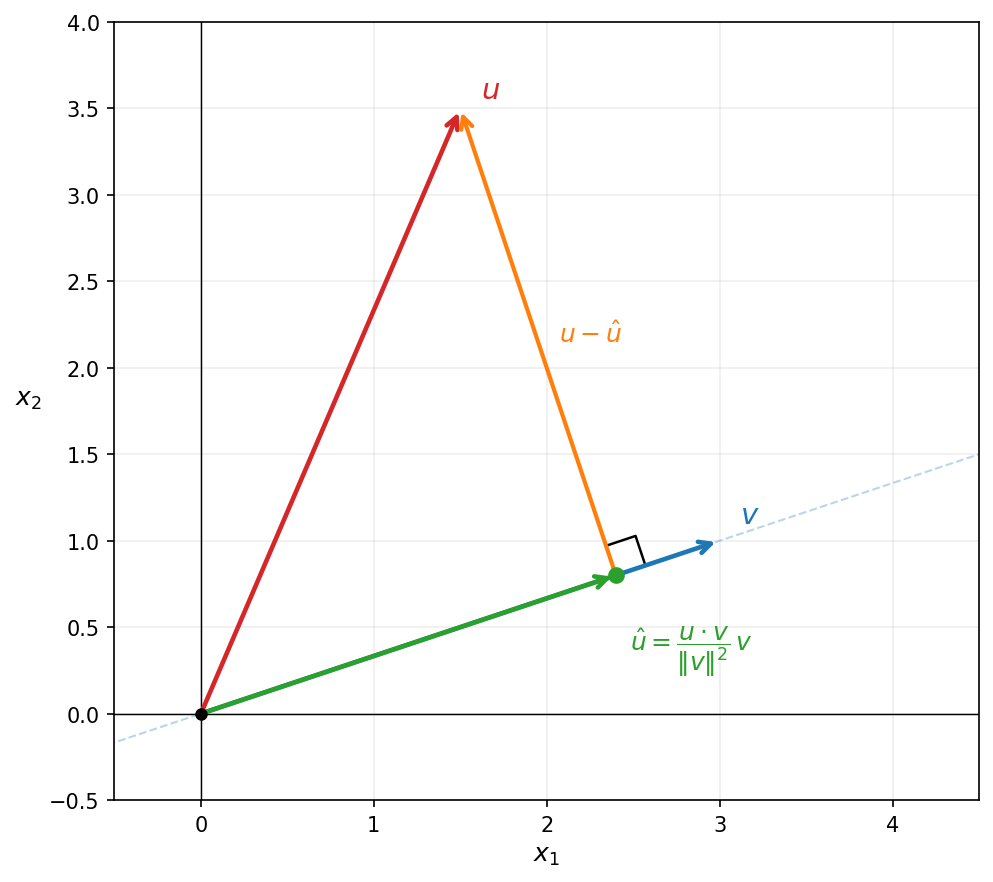
\includegraphics[width=0.68\textwidth]{book/assets/figures/core/fig04_projection.png}
  \caption{Projection splits $u$ into a part along $v$ and a residual
  perpendicular to $v$. This small picture is the prototype for least squares.}
\end{figure}

\begin{proposition}[Residual orthogonality]
If $v \neq 0$, then
\[
  u-\Proj_v(u) \perp v.
\]
\end{proposition}

\begin{proof}
\[
\begin{aligned}
  \inner{u-\Proj_v(u)}{v}
  &= \inner{u}{v}
     - \inner{\frac{\inner{u}{v}}{\inner{v}{v}}v}{v} \\
  &= \inner{u}{v}
     - \frac{\inner{u}{v}}{\inner{v}{v}}\inner{v}{v} \\
  &= 0.
\end{aligned}
\]
\end{proof}

\begin{computebox}
Projection is a decomposition:
\[
  u = \underbrace{\Proj_v(u)}_{\text{explained by }v}
      +
      \underbrace{(u-\Proj_v(u))}_{\text{orthogonal residual}}.
\]
In regression, the role of ``the line spanned by $v$'' is played by the
column space of a feature matrix. The model explains the component inside that
column space; the residual is the part left over.
\end{computebox}

\section{Cauchy--Schwarz And Angle}

The dot product in $\R^2$ satisfies
\[
  \inner{u}{v} = \norm{u}\norm{v}\cos\theta.
\]
In a general inner product space we turn this around: Cauchy--Schwarz proves
that the quotient below is always between $-1$ and $1$, so it can be used as
the cosine of an angle.

\begin{theorem}[Cauchy--Schwarz]
For all $u,v \in V$,
\[
  |\inner{u}{v}| \leq \norm{u}\norm{v}.
\]
Equality holds if and only if one of the vectors is a scalar multiple of the
other.
\end{theorem}

\begin{proof}
If $v=0$, the statement is immediate. Suppose $v \neq 0$. Decompose $u$ into
its projection onto $v$ and its residual:
\[
  u = \Proj_v(u) + r,\qquad r \perp v.
\]
By the Pythagorean theorem,
\[
  \norm{u}^2
  = \norm{\Proj_v(u)}^2+\norm{r}^2
  \geq \norm{\Proj_v(u)}^2.
\]
Now
\[
  \norm{\Proj_v(u)}
  =
  \left|\frac{\inner{u}{v}}{\inner{v}{v}}\right|\norm{v}
  =
  \frac{|\inner{u}{v}|}{\norm{v}}.
\]
Thus $\norm{u}^2 \geq |\inner{u}{v}|^2/\norm{v}^2$, which is equivalent to
$|\inner{u}{v}| \leq \norm{u}\norm{v}$. Equality holds exactly when
$\norm{r}=0$, i.e. when $u$ lies on the line spanned by $v$.
\end{proof}

\begin{definition}[Cosine similarity]
For nonzero vectors $u,v$ in an inner product space,
\[
  \cos(u,v)=\frac{\inner{u}{v}}{\norm{u}\norm{v}}.
\]
\end{definition}

Cosine similarity is common in data analysis because it ignores scale. If
$u$ and $10u$ represent the same direction with different magnitude, their
cosine similarity with another vector is the same.

\section{The Triangle Inequality}

\begin{theorem}[Triangle inequality]
For all $u,v \in V$,
\[
  \norm{u+v} \leq \norm{u}+\norm{v}.
\]
\end{theorem}

\begin{proof}
Using Cauchy--Schwarz,
\[
\begin{aligned}
  \norm{u+v}^2
  &= \norm{u}^2 + 2\inner{u}{v} + \norm{v}^2 \\
  &\leq \norm{u}^2 + 2|\inner{u}{v}| + \norm{v}^2 \\
  &\leq \norm{u}^2 + 2\norm{u}\norm{v} + \norm{v}^2 \\
  &= (\norm{u}+\norm{v})^2.
\end{aligned}
\]
Taking square roots gives the result.
\end{proof}

\section{Python Thread}

\begin{lstlisting}
import numpy as np

def dot(u, v):
    return float(u @ v)

def norm(u):
    return np.sqrt(dot(u, u))

def project_onto(u, v):
    return (dot(u, v) / dot(v, v)) * v

def cosine_similarity(u, v):
    return dot(u, v) / (norm(u) * norm(v))

u = np.array([3.0, 4.0])
v = np.array([1.0, 1.0])

p = project_onto(u, v)
r = u - p

print("projection:", p)
print("residual:", r)
print("residual dot v:", dot(r, v))
print("Pythagorean check:", np.allclose(norm(u)**2, norm(p)**2 + norm(r)**2))
print("cosine similarity:", cosine_similarity(u, v))
\end{lstlisting}

The numerical test is not a proof. It is a useful habit: when the theorem says
a residual is orthogonal, the code should make the corresponding dot product
close to zero.

\begin{labbox}
Lab 6 uses these ideas to implement Gram--Schmidt and to connect orthogonal
bases with QR factorization. The only required Python tools are arrays, matrix
multiplication, norms, and basic functions from \texttt{np.linalg}.
\end{labbox}

\section*{Chapter Summary}
\addcontentsline{toc}{section}{Chapter Summary}

\begin{itemize}
  \item An inner product adds geometry to a vector space.
  \item The induced norm measures length; distance is the norm of a difference.
  \item Orthogonality means inner product zero.
  \item Projection onto a line decomposes a vector into an explained part and
        an orthogonal residual.
  \item Cauchy--Schwarz justifies cosine similarity and powers the triangle
        inequality.
\end{itemize}

\section*{Exercises}
\addcontentsline{toc}{section}{Exercises}

\subsection*{A. Theory}

\begin{exercise}
\exerciseid{7.A1}
Let $v\neq 0$. Prove directly from the formula
$\Proj_v(u)=\frac{\inner{u}{v}}{\inner{v}{v}}v$ that
$u-\Proj_v(u)$ is orthogonal to $v$.
\end{exercise}

\begin{exercise}
\exerciseid{7.A2}
Prove the parallelogram identity:
\[
  \norm{u+v}^2+\norm{u-v}^2=2\norm{u}^2+2\norm{v}^2.
\]
\end{exercise}

\subsection*{B. By Hand}

\begin{exercise}
\exerciseid{7.B1}
Project $v=(3,4)$ onto the line spanned by $u=(1,1)$. Compute the residual
and check the dot product with $u$.
\end{exercise}

\begin{exercise}
\exerciseid{7.B2}
In $\R^2$, use the weighted inner product
\[
  \inner{x}{y}_w=x_1y_1+4x_2y_2.
\]
Compute the lengths of $a=(2,1)$ and $b=(2,-1)$, then check whether they are
orthogonal under this weighted inner product.
\end{exercise}

\subsection*{C. Python / NumPy}

\begin{exercise}
\exerciseid{7.C1}
Write a function that computes cosine similarity between two nonzero vectors.
Test it on two parallel vectors and two orthogonal vectors.
\end{exercise}

\begin{exercise}
\exerciseid{7.C2}
Generate 1000 random pairs of vectors in $\R^5$. For each pair, compute
\[
  \frac{|\inner{u}{v}|}{\norm{u}\norm{v}}.
\]
Use \texttt{np.max} to check that the largest observed value is at most $1$
up to floating-point error.
\end{exercise}

\subsection*{D. Challenge}

\begin{exercise}
\exerciseid{7.D1}
Give two different inner products on $\R^2$ for which the same two nonzero
vectors have different cosine similarities.
\end{exercise}

